\section{The TOV equation}
\label{section: TOV equation}

We will model a star as being made up of a \emph{perfect fulid}, which is entirely described by its energy density $u$ and pressure $p$.
The relationship between the pressure and energy density of a substance is called the \emph{equation of state}, or EOS, and has the form
\begin{equation}
    \label{EOS}
    f(p, u, \{\xi_i\}) = 0,
\end{equation}
where $\{\xi_i\}$ are possible other thermodynamic variables.
We will be working at zero temperature, in which case there are no other free thermodynamic variables.
This allows us to, at least locally, express the energy density as a function of the pressure, $u = u(p)$.
The stress-energy tensor of a perfect fluid is\todo{Forklar}
%
\begin{equation}
    T_{\mu \nu} = (u + p) u_\mu u_\nu - p g_{\mu \nu},
\end{equation} 
where $u_\mu$ is the 4-velocity of the fluid.
In the rest frame of the fluid, we may write 
\begin{equation}
    v_\mu = \left(v_0, 0, 0, 0\right).
\end{equation}
This, together with the normalization condition of 4-velocities, $v_\mu v^\mu = 1$, allows us to calculate that
%
\begin{equation}
    v_\mu v^\mu = g^{\mu \nu} v_\mu v_\nu = g^{00} (v_0)^2 = 1.
\end{equation}
%
Using \autoref{spherically symmetric metric}, we see that
\begin{equation}
    v_0 = e^{\alpha(r)}.
\end{equation}
%
This gives us the stress-energy tensor of the perfect fluid in its rest frame,
%
\begin{equation}
    T_{\mu \nu} 
    =
    \left(
        \begin{matrix}
            u{\left(r \right)} e^{2 \alpha{\left(r \right)}} & 0 & 0 & 0\\0 & 
            p{\left(r \right)} e^{2 \beta{\left(r \right)}} & 0 & 0\\
            0 & 0 & p{\left(r \right)} r^{2} & 0\\
            0 & 0 & 0 & p{\left(r \right)} r^{2} \sin^{2}{\left(\theta \right)}
        \end{matrix}
    \right).
\end{equation}
%
We will use the $tt$ and $rr$ components of the Einstein field equations, which are
%
\begin{align}
    \label{tt equation}
    8 \pi G r^{2} u{\left(r \right)} e^{2 \beta{\left(r \right)}} 
    & =   2 r \frac{d}{d r} \beta{\left(r \right)} + e^{2 \beta{\left(r \right)}} - 1 \\
    \label{rr equation}
    8 \pi G r^{2} p{\left(r \right)} e^{2 \beta{\left(r \right)}} 
    & = 2 r \frac{d}{d r} \alpha{\left(r \right)} - e^{2 \beta{\left(r \right)}} + 1.
\end{align}
%
In analogy with the Schwarzschild metric, we define the function $m(r)$ by
%
\begin{equation}
    e^{2 \beta(r)} = \left(1 - \frac{2 G m(r)}{r} \right)^{-1}. 
\end{equation}
%
Substituting this into \autoref{tt equation} yields 
%
\begin{equation}
    \label{diff eq mass}
    \odv{m(r)}{r} = 4 \pi r^2 \, u(r).
\end{equation}
%
The solution is simply
%
\begin{equation}
    \label{mass relation}
    m(r) = 4 \pi \int_0^r \dd r' \, {r'}^2 u(r').
\end{equation}
%
We see that $m(r)$ is the matter content contained within a radius $r$.
\todo{Forlar forskjell på gravitasjons masse/ incl. bindingsenergi}
If $u = 0$ for $r > R$ and $m(r>R) = M$, then the metric on a constant-time surface, i.e. $\dd t = 0$, is
%
\begin{equation}
    \dd s^2
    = 
    \left( 1 - \frac{2 G M}{r^2} \right)^{-1} \dd r^2 
    + r^2 (\dd \theta^2 + \sin^2 \theta \, \dd\varphi^2).
\end{equation} 
%
This is the same as for the Schwarzschild solution.

Using the Bianchi identity, \autoref{Einstein tensor bianchi identity}, together with Einstein's equation, we find
%
\begin{equation}
    \nabla^\mu G_{\mu \nu} = \nabla^\mu T_{\mu \nu} = 0.
\end{equation}
%
The $r$-component of this equation is
%
\begin{align*}
    \nabla_\mu T^{\mu r} 
    & =
    \partial_r T^{rr} 
    + \Gamma^\mu_{\mu \nu} T^{\nu r} 
    + \Gamma^r_{\mu \nu} T^{\mu \nu}\\
    & = 
    \partial_r \left(p e^{-2\beta}\right)
    + (2 \Gamma^r_{rr} + \Gamma^t_{tr}) T^{rr} 
    + \Gamma^r_{tt}T^{tt} \\ 
    &=   e^{-2\beta} \left( \partial_r p + p \partial_r \alpha + u \partial_r \alpha \right) = 0.
\end{align*} 
%
This allows us to relate $\alpha$ to $p$ and $u$, via
\begin{equation}
    \partial_r \alpha = - \frac{\partial_r p}{p + u}
\end{equation}
%
When we substitute this, together with the definition of $m(r)$, into \autoref{rr equation}, we obtain
%
\begin{equation}
    \label{TOV}
    \odv{p}{r}
    =
    -
    \frac{G}{r^2} 
    \left(4 \pi r^{3} p + m \right) 
    \left(p + u\right)
    \left(1 - \frac{2 G m}{r}\right)^{-1},
\end{equation}
%
the Tolman-Oppenheimer-Volkoff (TOV) equation.
This equation was first obtained by Oppenheimer and Volkoff in 1939~\autocite{oppenheimerMassiveNeutronCores1939} and was based on earlier work by Tolman~\autocite{tolmanRelativityThermodynamicsCosmology1934}.
In their paper, Oppenheimer and Volkoff studied the properties of a star made up of cold, degenerate fermions.

To summarize, we have three unknown functions, $u(r)$, $p(r)$, and $m(r)$.
The equation of state, \autoref{EOS}, determines $u = u(p)$, eliminating one unknown.
The two differential equations \autoref{mass relation} and \autoref{TOV}, together with the boundary conditions $p(0) = p_c$ and $m(0) = 0$, then yield $p(r)$ and $m(r)$ when integrated.
Given this, we can solve for all the unknown functions, either analytically or numerically.
However, we can gain some insight into the system without solving these equations by expressing the problem in terms of dimensionless variables.
We define
%
\begin{equation}
    u = u_0 \tilde u, \quad 
    p = p_0 \tilde p, \quad 
    m = m_0 \tilde m, \quad 
    r = r_0 \tilde r.
\end{equation}
%
Here, quantities with subscript $0$ are dimensionful constants, which may be chosen as the characteristic quantities of the problem, while the tilde indicates a dimensionless variable.
By substituting this into \autoref{diff eq mass} and \autoref{TOV}, we can collect the dimensionful constants into a smaller number of dimensionless constants, $k_i$.
These constants will decide the nature of the solution.
Any change in the dimensionful constants that leave the $k_i$'s invariant is a scaling of the problem --- it corresponds to the same solution with different units.
The new differential equations are
%
\begin{align}
    \label{mass relation dimensionless}
    \odv{ \tilde m}{\tilde r} & = 3 k_2\, \tilde r^2 \tilde u \\
    \label{TOV dimensionless}
    \odv{\tilde p}{\tilde r} & 
    = - \frac{k_1}{k_3} \frac{1}{\tilde r^2} \left(k_3\tilde p + \tilde u\right) 
    \left(3 k_2 k_3  \tilde r^3 \tilde p + \tilde m\right) 
    \left(1 - \frac{2 k_1  \tilde m}{\tilde r}\right)^{-1},
\end{align}
%
where the dimensionless constants are defined as
%
\begin{equation}
    \label{dimensionless constants TOV}
    k_1 = G \frac{m_0}{r_0}, \quad 
    k_2 =  \frac{4 \pi}{3} \frac{r_0^3 u_0}{m_0}, \quad
    k_3 = \frac{p_0}{u_0}.
\end{equation}
%
The energy density and pressure are of comparable magnitude in the relativistic regime.
We will therefore often choose $k_3 = 1$, defining $p_0 = u_0$.
If we have a non-complete set of characteristic quantities, the dimensionless constants $k_i$ tell us something about the magnitude we should expect the solution to have.
After defining the remaining dimensionful constants by setting $k_i = 1$, we expect that the dimensionless sizes of a typical solution will be of order 1.
In other words, the dimensionful constants defined by $k_i = 1$ are new, characteristic quantities given to us by the form of the governing equation only.


\subsection{Newtonian limit}

In the Newtonian limit, the rest energy, i.e., mass, gives the dominant contribution to the gravitational field, while the contribution from pressure is negligible. 
In other words, the characteristic pressure, $p_0$, is far smaller than the characteristic energy density $u_0$, and we can use the approximation $k_3 \ll 1$.
Furthermore, the star's radius should be much larger than the Schwarzschild radius, $R_s = 2 G M$.
If we choose $r_0 = R$, then $ k_1 \ll 1$.
In this limit, the lowest-order contribution to the TOV equation is
%
\begin{equation}
    \label{Newtonian limit TOV}
    \odv{\tilde p}{\tilde r} = - \frac{k}{\tilde r^2}\tilde u \tilde m, \quad
    k = \frac{k_1}{k_3} =  G \frac{u_0 m_0}{p_0 r_0}.
\end{equation}
%
Using the mass equation \autoref{mass relation dimensionless}, we can write this as
%
\begin{equation}
    4 \pi \tilde r^2 \odv{\tilde p}{\tilde m}
    = - k' \frac{\tilde m}{\tilde r^2}, 
    \quad k' = \frac{4 \pi}{3} \frac{k_1}{k_2 k_3} = G \frac{m_0^2}{r_0^4 p_0}.
\end{equation}
%
We may derive this equation directly from Newtonian gravity.
Assume we have a static, gravitationally bound ball of matter, as illustrated in \autoref{fig: hydrostatic equillibrium}.
The force due to the pressure gradient over a thin, spherical shell, $F_p = 4 \pi r^2 \dd p$, must be counteracted by the gravitational force on the same shell, $F_g = - G m \dd m / r^2$.

\begin{figure}[h]
    \centering
    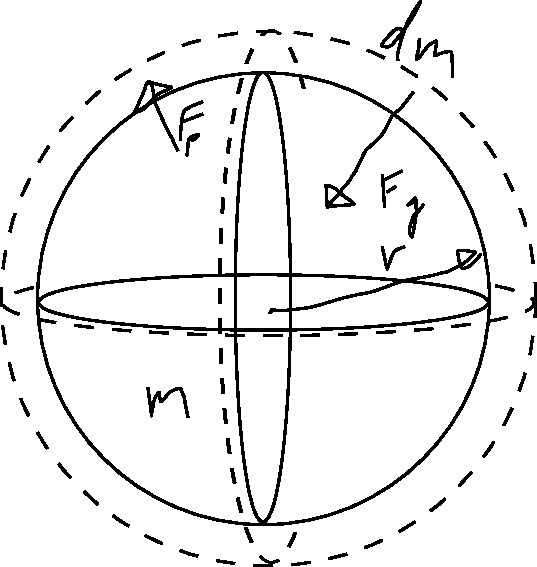
\includegraphics[width=0.32\textwidth]{figurer/hydrostatic_equillibrium.pdf}
    \caption{Kladd: The forces acting on a thin shell $\dd m$.}
    \label{fig: hydrostatic equillibrium}
\end{figure}

Both the Newtonian limit and the TOV equation are equations of \emph{hydrostatic equilibrium}, where the forces on a small volume of the fluid cancel out.
In the case of the TOV equation, we tacitly assumed hydrostatic equilibrium when we gave the fluid a rest frame where we could write $v_\mu = (v_0, 0, 0, 0)$ globally.
We can eliminate the equation for mass by differentiating \autoref{Newtonian limit TOV} with respect to $\tilde r$.
This gives us a single equation for hydrostatic equilibrium in the Newtonian limit,
%
\begin{equation}
    \odv{}{\tilde r} 
    \left( \frac{\tilde r^2}{\tilde u} \odv{\tilde p}{\tilde r}\right) 
    = -  k'' \tilde r^2  \tilde u, \quad
    k'' = 3 \frac{k_2 k_1}{k_3} = 4 \pi G \frac{u_0^2 r^2_0}{p_0}.
\end{equation}



\subsection{Incompressible fluid}

The simplest model for a star is one made up of an incompressible fluid, where the energy density is independent of the pressure.
In this case, the energy density of the star will be constant for a radius $r < R$, before it drops to zero,
%
\begin{equation}
    u(r) = u_0 \, \theta (R- r),
\end{equation}
%
where $u_0$ is a constant and $\theta(x)$ the Heaviside step function.
We choose $r_0 = R$.
Inserting this into the differential equation of the mass function, \autoref{mass relation dimensionless}, together with the boundary condition $m(0) = 0$, yields
%
\begin{equation}
    \tilde m(\tilde r) = k_2 \tilde r^3,
\end{equation}
%
when $r < R$.
For $r \geq R$, or $\tilde r \geq 1$, this relationship is simply constant $\tilde m(\tilde r) = \tilde m(1) = k_2$.
We choose $m_0$ to be the gravitational mass of the star, $M = \frac{4 \pi }{3} R^3 u_0$, which is equivalent to setting $k_2 = 1$.
Lastly, we choose $u_0 = p_0$, so that $k_3 = 1$.
With this the TOV equation, \autoref{TOV dimensionless}, becomes
%
\begin{equation} 
    \odv{\tilde p}{\tilde r} 
    = - k_1 \tilde r 
    \frac{(1 + \tilde p)(1 + 3 \tilde p)}{(1 - 2 k_1 \tilde r^2)}.
\end{equation}
%
This is a separable ODE, and each variable may be integrated separately.
Using
%
\begin{align}
    \int \frac{\dd x}{(1 + x)(1 + 3x)}
    = \frac{1}{2} \ln \frac{3x + 1}{x + 1} + \const , \quad
    \int \dd x \frac{x}{1 - 2 x^2} 
    = \frac{1}{4}\ln\left(1 - 2 x^2 \right)
    + \const,
\end{align}
%
together with the boundary condition $p(r = R) = 0$, we get 
%
\begin{equation}
    \label{pressure afo r incompressible}
    \tilde p(\tilde r) 
    = 
    - \frac{\sqrt{1 - 2 k_1} - \sqrt{1 - 2 k_1 \tilde r^2}}
    {3 \sqrt{1 - 2 k_1 } - \sqrt{1 - 2 k_1 \tilde r^2}}.
\end{equation}
%
We see that the star is entirely characterized by $k_1$.
In \autoref{fig: pressure incompressible fluid}, we have plotted the pressure as a function of radius for some values of $k_1$.
As $k_1$ approaches $0.\bar 4 = 4/9$, the pressure at the center of the star increases rapidly.
From the denominator of \autoref{pressure afo r incompressible} at $r\rightarrow 0$, we find the limit
%
\begin{equation}
    \label{mass radius constraint}
    k_1 = G \frac{M}{R} < \frac{4}{9}
\end{equation}
%
for the pressure to remain finite.
This is an absolute limit of the mass of an object given its radius or vice versa.
Although this limit is derived for a particular, unrealistic case, the more general statement can be shown to hold.
General relativity does not allow for a static solution with energy densities greater than this limit; any such configuration would collapse~\autocite{carrollSpacetimeGeometryIntroduction2019}.


\begin{figure}[h]
    \centering
    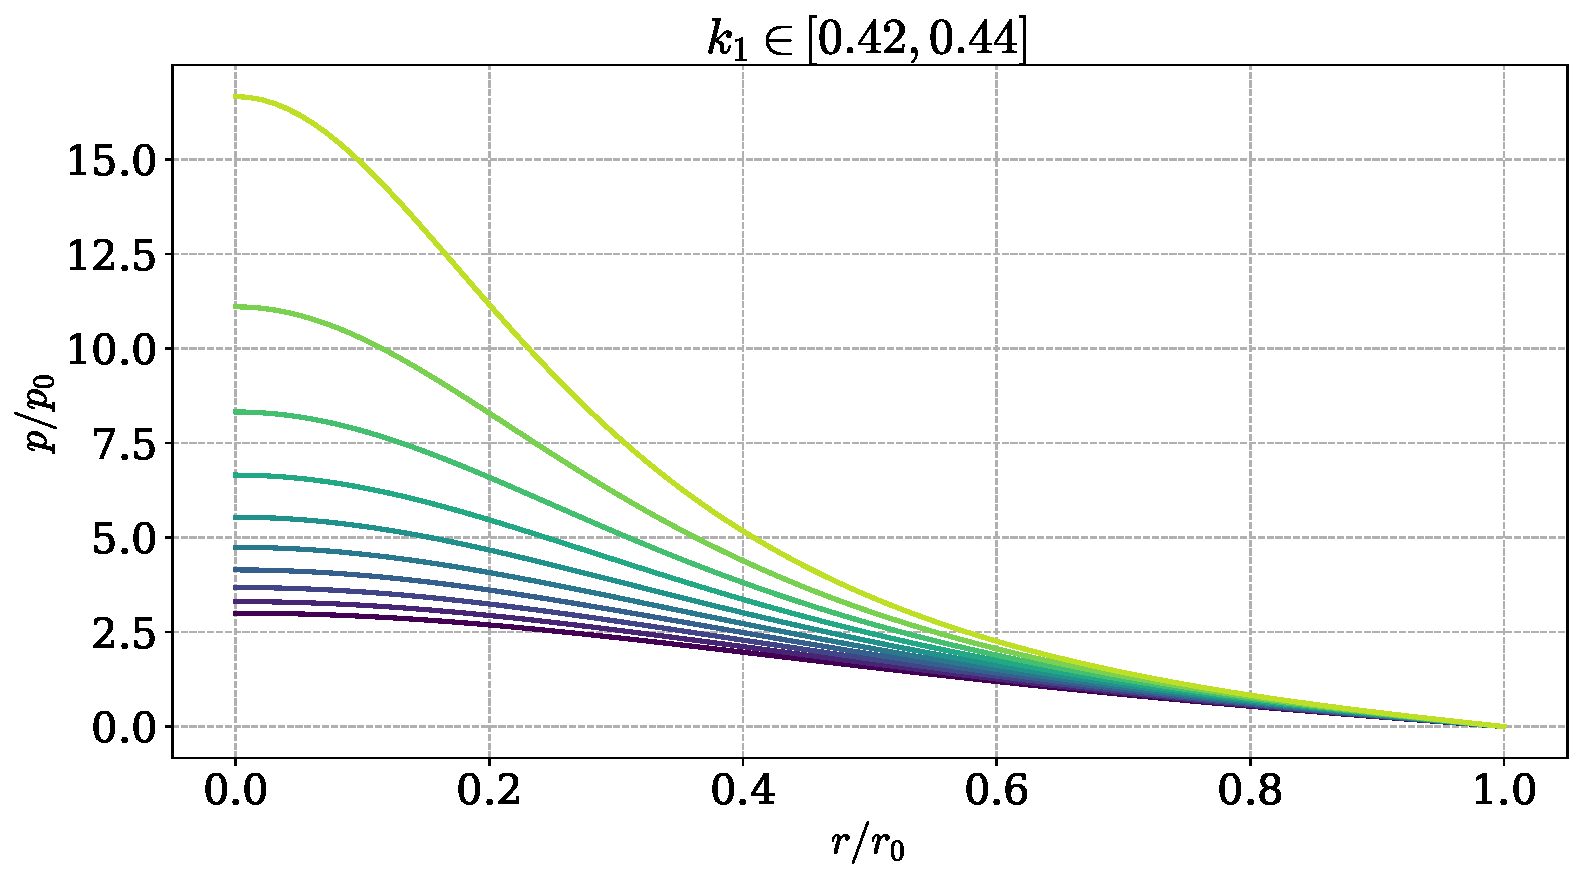
\includegraphics[width=0.8\textwidth]{../scripts/figurer/incompressible.pdf}
    \caption{The pressure in units of $p_0$, as a function of the radius, in units of $r_0$. The graphs with lighter color and higher pressure at $r = 0$ corresponds to higher values of $k_1$. The values of $k_1$ are linearly spaced.}
    \label{fig: pressure incompressible fluid}
\end{figure}

 
If we expand the solution \autoref{pressure afo r incompressible} in powers of $k_1$, then the leading order contribution is
%
\begin{equation}
    \tilde p(r) = \frac{1}{2} k_1 (1 - \tilde r^2).
\end{equation}
%
This is the Newtonian limit.
As a cross-check, we see that this solution obeys the equation of hydrostatic equillibrium in this limit, \autoref{Newtonian limit TOV}, as $\tilde u = 1$ and $k_2 = k_1 = 1$.
This is the general solution for an incompressible fluid in Newtonian gravity.
This solution does not have any upper limit for $k_1$; the limit $M/R < 4 / 9$ is purely relativistic phenomenon.
In \autoref{fig: pressure incompressible fluid newtonian}, the Newtonian approximation is compared to the full, relativistic solution.
We see that the Newtonian approximation is highly accurate for $k_1$ less than around $0.01$.


\begin{figure}[h]
    \centering
    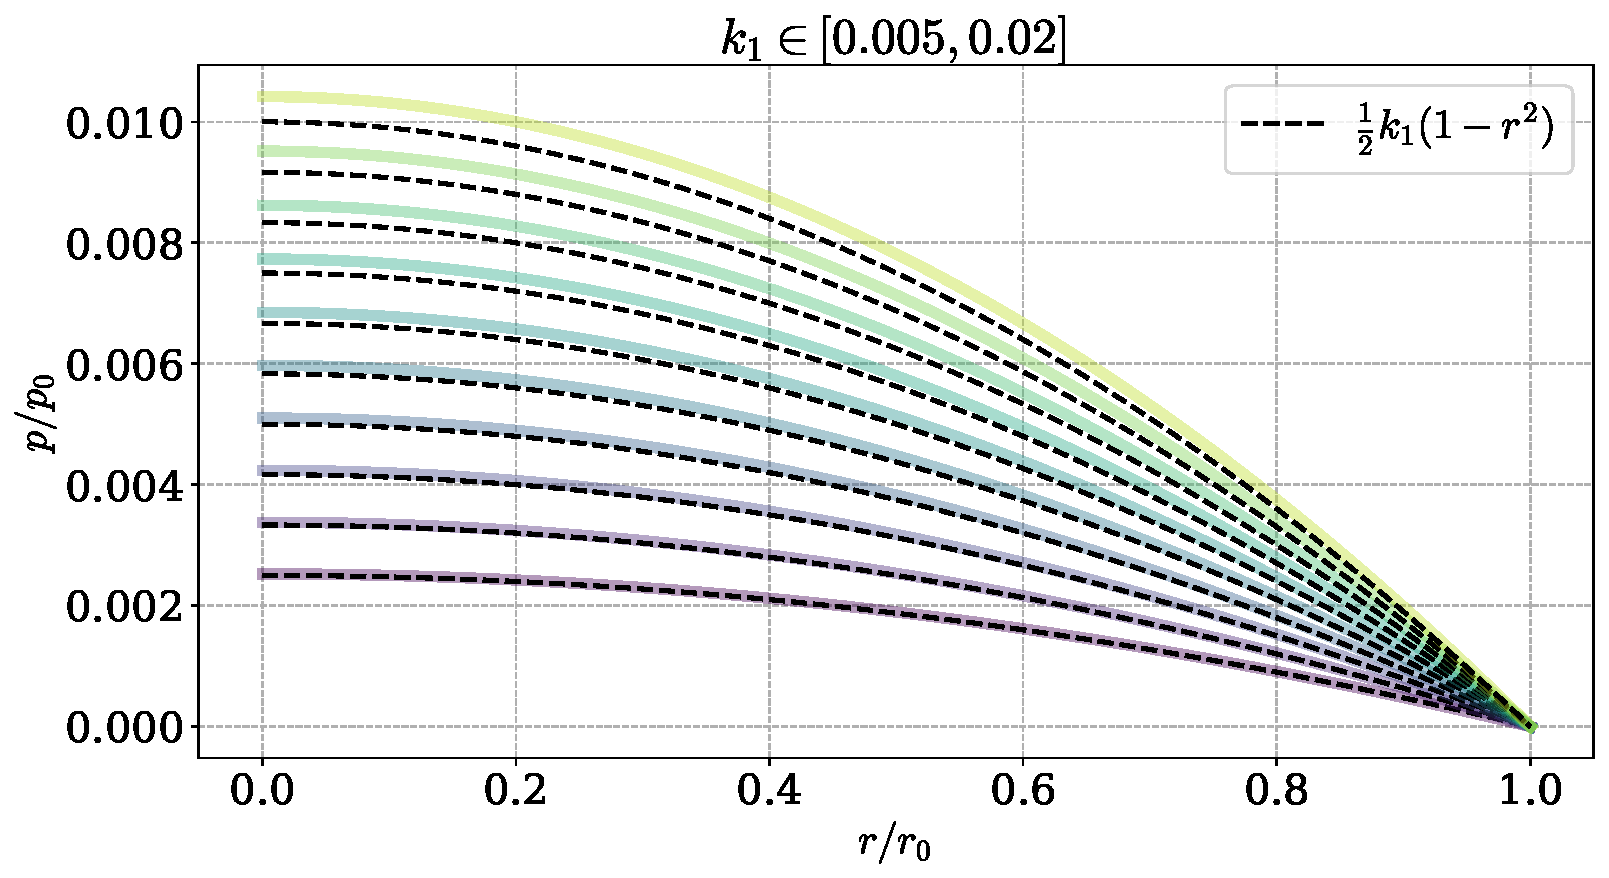
\includegraphics[width=0.8\textwidth]{../scripts/figurer/incompressible_newt.pdf}
    \caption{The pressure in units of $p_0$, as a function of the radius, in units of $r_0$. The wide, colored lines correspond to the full relativistic solution, while the dashed lines is the Newtonian approximation, for the same value of $k_1$. The values of $k_1$ are linearly spaced.  }
    \label{fig: pressure incompressible fluid newtonian}
\end{figure}

